\documentclass{article}
\usepackage[utf8]{inputenc}
\usepackage{amsmath}
\usepackage{amssymb}
\usepackage{tkz-graph}
\tikzset{EdgeStyle/.append style = {->} }
\renewcommand{\thesubsection}{\alph{subsection})}
\title{Osztott rendszerek szintézise\\7. tétel}
\begin{document}
%\maketitle

\section*{Legrövidebb út}
\subsection{Specifikáció és megoldások: szekvenciális megoldás, megoldás egyenlőségi sémában és szinkron közös memóriás architektúrán}
\subsubsection*{Specifikáció}
\begin{align*}
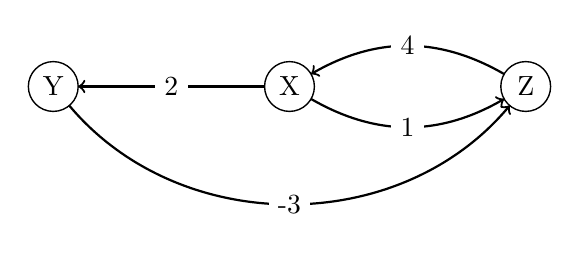
\begin{tikzpicture}
  \SetGraphUnit{3}
  \Vertex{X}
  \WE(X){Y}
  \EA(X){Z}
  \Edge[label = 2](X)(Y)
  \tikzset{EdgeStyle/.append style = {bend right}}
  \Edge[label = 1](X)(Z)
  \Edge[label = 4](Z)(X)
  \tikzset{EdgeStyle/.append style = {bend right = 50}}
  \Edge[label = -3](Y)(Z)
\end{tikzpicture}
\end{align*}
---------------------------------------------------------------------------------------------------
\begin{align*}
\begin{tabular}{c|c|c|c}
  & X & Y & Z  \\ \hline
X & 0 & 2 & 1 \\
Y & 1 & 0 & -3 \\
Z & 4 & 6 & 0 
\end{tabular}
\end{align*}
\subsection{megoldás aszinkron architektúrán és elosztott rendszerben}
\end{document}
